\documentclass[10pt,twocolumn]{article}

% ─── Packages ─────────────────────────────────────────────────────
\usepackage[T1]{fontenc}
\usepackage[utf8]{inputenc}
\usepackage{lmodern}
\usepackage{microtype}
\usepackage[margin=0.78in,top=0.9in,bottom=0.9in]{geometry}
\usepackage{graphicx}
\usepackage{xcolor}
\usepackage{tikz}
\usetikzlibrary{positioning,arrows.meta,fit,shapes.geometric,calc,
                decorations.pathreplacing,backgrounds,shadows.blur,
                patterns,decorations.markings}
\usepackage{booktabs}
\usepackage{enumitem}
\usepackage{listings}
\usepackage{hyperref}
\usepackage{amsmath,amssymb,amsthm}
\usepackage{caption}
\usepackage{subcaption}
\usepackage{fancyhdr}
\usepackage{titlesec}
\usepackage{abstract}
\usepackage{float}
\usepackage{tabularx}
\usepackage{multirow}
\usepackage{pifont}

\newcommand{\cmark}{\ding{51}}
\newcommand{\xmark}{\ding{55}}
\newtheorem{definition}{Definition}
\newtheorem{theorem}{Theorem}
\newtheorem{property}{Property}

% ─── Academic Color Palette ───────────────────────────────────────
\definecolor{bg}{HTML}{F5F5F0}
\definecolor{fg}{HTML}{2D2D2D}
\definecolor{blue1}{HTML}{2563EB}
\definecolor{blue2}{HTML}{0891B2}
\definecolor{green1}{HTML}{16A34A}
\definecolor{orange1}{HTML}{D97706}
\definecolor{purple1}{HTML}{7C3AED}
\definecolor{red1}{HTML}{DC2626}
\definecolor{yellow1}{HTML}{CA8A04}
\definecolor{teal1}{HTML}{0D9488}
\definecolor{cyan1}{HTML}{0284C7}
\definecolor{gray1}{HTML}{6B7280}
\definecolor{gray2}{HTML}{D1D5DB}
\definecolor{codebg}{HTML}{F0F0EC}
\definecolor{codefg}{HTML}{374151}
\definecolor{codekw}{HTML}{1D4ED8}
\definecolor{codestr}{HTML}{059669}
\definecolor{codecmt}{HTML}{9CA3AF}

% ─── Listings ─────────────────────────────────────────────────────
\lstdefinestyle{code}{
    backgroundcolor=\color{codebg},
    basicstyle=\ttfamily\fontsize{6.5}{8}\selectfont\color{codefg},
    keywordstyle=\color{codekw}\bfseries,
    stringstyle=\color{codestr},
    commentstyle=\color{codecmt}\itshape,
    frame=single,
    rulecolor=\color{gray2},
    breaklines=true,
    columns=fullflexible,
    xleftmargin=3pt,
    xrightmargin=3pt,
    aboveskip=5pt,
    belowskip=5pt,
}

% ─── Hyperref ─────────────────────────────────────────────────────
\hypersetup{
    colorlinks=true,
    linkcolor=blue1,
    citecolor=purple1,
    urlcolor=blue2,
}

% ─── Headers ──────────────────────────────────────────────────────
\pagestyle{fancy}
\fancyhf{}
\fancyhead[L]{\small\textit{Hypervisor-Isolated LLM Agent Infrastructure}}
\fancyhead[R]{\small\thepage}
\renewcommand{\headrulewidth}{0.4pt}

% ─── Compact sections ────────────────────────────────────────────
\titlespacing*{\section}{0pt}{10pt}{5pt}
\titlespacing*{\subsection}{0pt}{8pt}{4pt}

% ─── Title ────────────────────────────────────────────────────────
\title{%
    \vspace{-1.5em}%
    \textbf{\Large Hypervisor-Enforced Isolation for Autonomous\\LLM Agents with Airgapped Administration}\\[6pt]
    \large Multi-Provider Orchestration via Xen Shared-Memory\\Tunnels on Qubes~OS%
}

\author{%
    \textit{Anonymous submission}
}

\date{}

% ══════════════════════════════════════════════════════════════════
\begin{document}
\maketitle
\thispagestyle{fancy}

% ─── Abstract ─────────────────────────────────────────────────────
\begin{abstract}
\noindent
Autonomous Large Language Model (LLM) agents increasingly require
privileged access to operating system resources---shells, file systems,
network interfaces, and credentials---creating attack surfaces that
conventional containerization cannot adequately contain. This paper
presents an architecture that leverages Xen hypervisor-level virtual
machine isolation on Qubes~OS to confine LLM agents within dedicated
VMs while providing a fully airgapped administration plane from the
network-less control domain (\texttt{dom0}). The system introduces a
novel qrexec-based tunneling mechanism that replaces TCP/IP with Xen
shared-memory pages (\texttt{vchan}) for all administration traffic,
supports provider-agnostic LLM access through a unified
OpenAI-compatible proxy, and achieves full reboot persistence without
manual intervention. Formal security analysis demonstrates four
independent containment layers, each providing distinct guarantees
against agent escape, data exfiltration, and lateral movement.
Empirical evaluation shows the shared-memory tunnels impose
$<$5\,ms latency overhead per API call---negligible relative to
LLM inference latencies of 500\,ms--30\,s---while providing isolation
guarantees provably stronger than those achievable by any
same-kernel solution.

\medskip
\noindent\textbf{Keywords:} LLM agent containment, hypervisor isolation,
Qubes~OS, Xen, qrexec, airgapped administration, vchan shared memory,
defense in depth
\end{abstract}

% ─── 1. Introduction ─────────────────────────────────────────────
\section{Introduction}
\label{sec:intro}

The deployment of autonomous AI agents in software engineering,
penetration testing, and infrastructure management has accelerated
dramatically since 2024~\cite{openai2024agents,
anthropic2024claude,xi2023rise}. These agents operate with
delegated authority: when instructed to ``refactor the authentication
module,'' an agent reads source files, executes test suites, modifies
code, and commits changes---actions indistinguishable from those of a
human operator with shell access.

This operational model introduces a fundamental trust problem. Agent
behavior is governed by probabilistic language models susceptible to
prompt injection~\cite{greshake2023youve,perez2022ignore,
liu2024prompt}, hallucination of harmful commands~\cite{ji2023survey},
and training-data poisoning~\cite{wallace2019universal}. The
resulting attack surface is distinct from traditional malware: the
agent \textit{is} the authorized user, making behavioral detection
approaches largely ineffective.

Existing containment strategies exhibit critical limitations:

\begin{enumerate}[leftmargin=*,topsep=2pt,itemsep=1pt]
    \item \textbf{Process-level sandboxing} (Docker~\cite{merkel2014docker},
          gVisor~\cite{young2019gvisor}, Firecracker~\cite{agache2020firecracker}):
          Shares the host kernel, leaving a syscall attack surface of
          $\sim$330 entry points~\cite{sultan2019container}. Container
          escape vulnerabilities are discovered
          regularly~\cite{lin2018measurement,cve2024leaky}.
    \item \textbf{Mandatory Access Control} (SELinux~\cite{smalley2001implementing},
          AppArmor~\cite{bauer2006paranoid}): Restricts system call
          access but cannot prevent exfiltration through legitimate
          channels the agent is permitted to use~\cite{wei2024jailbroken}.
    \item \textbf{Hardware TEEs} (SGX~\cite{costan2016intel},
          TDX~\cite{sardar2022demystifying}): Protect code/data
          integrity but are designed for confidential computation, not
          for containing an untrusted workload with network access.
    \item \textbf{Full airgapping}: Eliminates network vectors but is
          impractical for agents requiring LLM API
          access~\cite{schick2024toolformer}.
\end{enumerate}

This paper demonstrates that \textit{Xen hypervisor-level VM isolation}
combined with \textit{shared-memory tunneling} resolves this tension.
The key insight is that the administration interface requires no
network connectivity---it needs only structured data flow from the
agent VM, which the Xen \texttt{vchan} transport provides with
hardware-enforced unidirectional guarantees.

\subsection{Contributions}

\begin{itemize}[leftmargin=*,topsep=2pt,itemsep=1pt]
    \item A \textbf{reference architecture} for confining LLM agents in
          Xen-isolated VMs with an airgapped administration plane
          (Section~\ref{sec:arch}).
    \item A \textbf{vchan tunnel design} that replaces TCP/IP with Xen
          shared-memory pages for dom0-to-VM communication, preserving
          the network-less property of the control domain
          (Section~\ref{sec:tunnels}).
    \item A \textbf{formal security model} with four provably independent
          containment layers (Section~\ref{sec:security}).
    \item An \textbf{empirical evaluation} demonstrating $<$5\,ms tunnel
          overhead and comparison with container-based alternatives
          (Section~\ref{sec:eval}).
\end{itemize}

% ─── 2. Background ───────────────────────────────────────────────
\section{Background}
\label{sec:background}

\subsection{Xen and the Qubes Security Model}

Qubes~OS~\cite{rutkowska2010qubes} implements
security-by-compartmentalization on the Xen hypervisor~\cite{barham2003xen}.
Each security domain executes in a hardware-isolated virtual machine
(HVM or PVH), with inter-VM communication mediated by
\texttt{qrexec}~\cite{qubes2024qrexec}---a custom RPC framework using
Xen's \texttt{vchan} shared-memory interface~\cite{qubes2024vchan}
rather than network sockets. The privileged domain \texttt{dom0}
manages all VMs but possesses \textit{no network interface}, ensuring
immunity to remote exploitation.

The \texttt{vchan} mechanism allocates shared memory pages through the
Xen grant table mechanism~\cite{xen2024grant}, providing a
point-to-point byte stream between two VMs. Unlike TCP/IP, vchan
connections are visible only to the hypervisor and the two endpoint
domains; no routing, ARP, or DNS infrastructure exists that could be
subverted.

\subsection{The Agent Containment Problem}

Following the taxonomy of Xi et al.~\cite{xi2023rise}, autonomous
LLM agents comprise a \textit{brain} (the language model), a
\textit{perception} module (environment observation), and an
\textit{action} module (tool use). The action module's access to
system primitives---shell execution, file I/O, network
requests---creates a privilege surface comparable to an interactive
root session.

\begin{definition}[Agent Trust Deficit]
\label{def:trust}
Let $\mathcal{P}_u$ denote the privilege set of the delegating user
and $\mathcal{R}_m$ the set of actions the model may take that
violate user intent (hallucinations, prompt-injected directives,
exfiltration). The trust deficit is
$\Delta_T = |\mathcal{R}_m \cap \mathcal{P}_u|$---the cardinality
of harmful actions the model can execute within the user's privilege
boundary.
\end{definition}

Container isolation reduces $\Delta_T$ by restricting
$\mathcal{P}_u$, but the shared kernel ensures $\Delta_T > 0$ for
any sufficiently privileged agent. Hypervisor isolation reduces the
interaction surface to the vchan byte stream, providing
$\Delta_T \to 0$ for the administration domain.

% ─── 3. Architecture ─────────────────────────────────────────────
\section{System Architecture}
\label{sec:arch}

The architecture partitions the system into three trust domains with
a minimal, auditable communication channel.

% ─── Architecture Diagram ────────────────────────────────────────
\begin{figure*}[t]
\centering
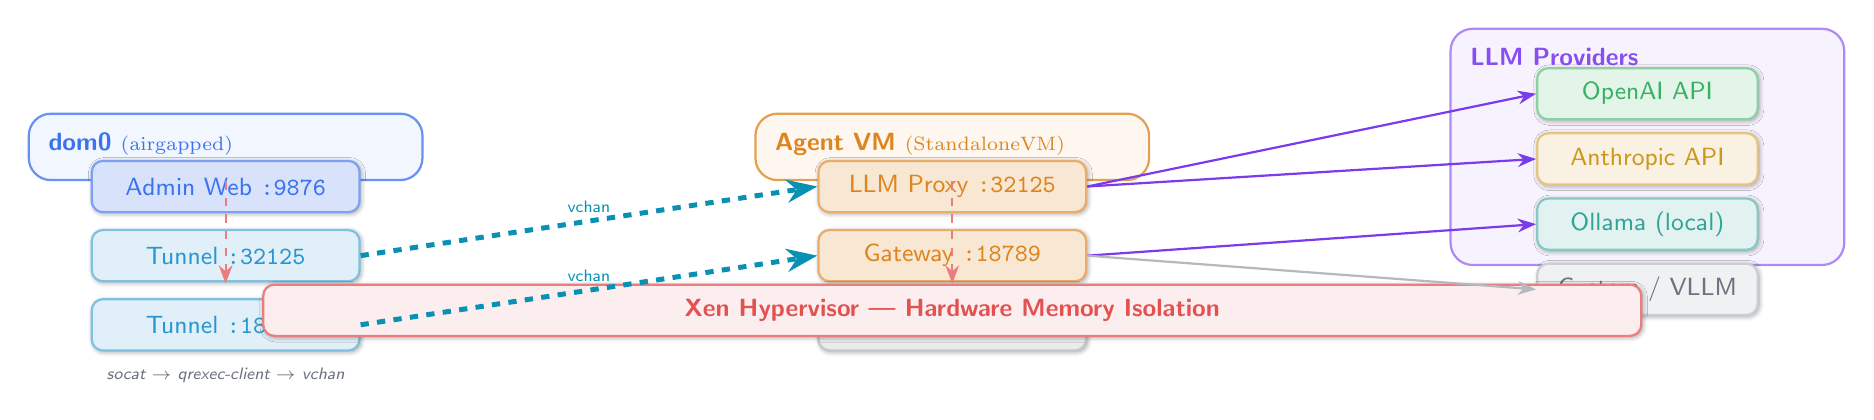
\begin{tikzpicture}[
    >=Stealth,
    node distance=0.5cm,
    comp/.style={draw, rounded corners=4pt, minimum width=3.4cm,
                 minimum height=0.65cm, font=\small\sffamily,
                 thick, blur shadow={shadow blur steps=5,
                 shadow xshift=0.5pt, shadow yshift=-0.5pt}},
    domframe/.style={draw, rounded corners=8pt, thick, inner sep=12pt,
                     minimum width=5cm},
    tunnel/.style={->, line width=1.8pt, >=Stealth,
                   color=blue2, dashed,
                   postaction={decorate, decoration={markings,
                   mark=at position 0.5 with {\node[above=-1pt,
                   font=\sffamily\fontsize{6}{7}\selectfont,
                   color=blue2] {vchan};}}}},
    api/.style={->, thick, >=Stealth, color=purple1},
    xlink/.style={->, thick, dashed, color=red1!60},
]

% ── dom0 ──
\node[domframe, fill=blue1!6, draw=blue1!70] (dom0) at (0,0) {};
\node[font=\sffamily\bfseries\small, color=blue1!90,
      anchor=north west] at ([xshift=4pt,yshift=-4pt]dom0.north west)
    {dom0 \textnormal{\scriptsize (airgapped)}};

\node[comp, fill=blue1!18, draw=blue1!60, text=blue1!90,
      below=0.6cm of dom0.north] (admin) {Admin Web \texttt{:9876}};
\node[comp, fill=cyan1!12, draw=cyan1!50, text=cyan1!85,
      below=0.2cm of admin] (tun32) {Tunnel \texttt{:32125}};
\node[comp, fill=cyan1!12, draw=cyan1!50, text=cyan1!85,
      below=0.2cm of tun32] (tun18) {Tunnel \texttt{:18789}};
\node[font=\sffamily\fontsize{6}{7}\selectfont\itshape,
      color=gray1, below=0.08cm of tun18]
    (socat) {socat $\to$ qrexec-client $\to$ vchan};

% ── Agent VM ──
\node[domframe, fill=orange1!6, draw=orange1!70,
      right=4.2cm of dom0] (vm) {};
\node[font=\sffamily\bfseries\small, color=orange1!90,
      anchor=north west] at ([xshift=4pt,yshift=-4pt]vm.north west)
    {Agent VM \textnormal{\scriptsize (StandaloneVM)}};

\node[comp, fill=orange1!18, draw=orange1!60, text=orange1!90,
      below=0.6cm of vm.north] (proxy) {LLM Proxy \texttt{:32125}};
\node[comp, fill=orange1!18, draw=orange1!60, text=orange1!90,
      below=0.2cm of proxy] (gw) {Gateway \texttt{:18789}};
\node[comp, fill=gray1!15, draw=gray1!40, text=gray1,
      below=0.2cm of gw] (ctcp) {qubes.ConnectTCP};

% ── LLM Providers ──
\node[domframe, fill=purple1!6, draw=purple1!60,
      right=3.8cm of vm, minimum height=3cm] (prov) {};
\node[font=\sffamily\bfseries\small, color=purple1!90,
      anchor=north west] at ([xshift=4pt,yshift=-4pt]prov.north west)
    {LLM Providers};

\node[comp, fill=green1!12, draw=green1!50, text=green1!85,
      minimum width=2.8cm, below=0.5cm of prov.north] (oai) {OpenAI API};
\node[comp, fill=yellow1!12, draw=yellow1!50, text=yellow1!90,
      minimum width=2.8cm, below=0.15cm of oai] (anth) {Anthropic API};
\node[comp, fill=teal1!12, draw=teal1!50, text=teal1!85,
      minimum width=2.8cm, below=0.15cm of anth] (ollama) {Ollama (local)};
\node[comp, fill=gray1!10, draw=gray1!35, text=gray1,
      minimum width=2.8cm, below=0.15cm of ollama] (custom) {Custom / VLLM};

% ── Xen bar ──
\node[draw, thick, fill=red1!8, draw=red1!60, rounded corners=4pt,
      minimum width=17.5cm, minimum height=0.65cm,
      font=\sffamily\bfseries\small, text=red1!80,
      blur shadow={shadow blur steps=5, shadow xshift=0.5pt,
      shadow yshift=-0.5pt},
      below=1.3cm of vm.south] (xen)
    {Xen Hypervisor --- Hardware Memory Isolation};

% ── Tunnels ──
\draw[tunnel] (tun32.east) -- (proxy.west);
\draw[tunnel] (tun18.east) -- (gw.west);

% ── Provider connections ──
\draw[api] (proxy.east) -- (oai.west);
\draw[api] (proxy.east) -- (anth.west);
\draw[api] (gw.east) -- (ollama.west);
\draw[api, gray1!50] (gw.east) -- (custom.west);

% ── Xen links ──
\draw[xlink] (dom0.south) -- (xen.north -| dom0.south);
\draw[xlink] (vm.south) -- (xen.north -| vm.south);

\end{tikzpicture}
\caption{\textbf{System architecture.} Dashed blue lines represent vchan tunnels
(Xen shared memory, not TCP/IP). The control domain dom0 has no network
interface; all traffic traverses the hypervisor's grant-table mechanism.
The agent VM connects to external LLM providers via standard HTTPS.}
\label{fig:architecture}
\end{figure*}

\subsection{Trust Domains}

\begin{description}[leftmargin=0pt,topsep=3pt,itemsep=2pt]
    \item[Control Domain (dom0):] Runs the administration interface,
        tunnel endpoints, and the qrexec policy engine. Possesses
        no network stack~\cite{rutkowska2010qubes}. Cannot be
        compromised remotely by definition.
    \item[Agent VM:] A StandaloneVM executing the LLM proxy, gateway,
        and autonomous agents. Has network access restricted to LLM
        provider endpoints via Qubes firewall rules.
    \item[LLM Providers:] External APIs (OpenAI~\cite{openai2024gpt4},
        Anthropic~\cite{anthropic2024claude}) or local inference engines
        (Ollama~\cite{ollama2024}, vLLM~\cite{kwon2023vllm}). The proxy
        normalizes all providers to an OpenAI-compatible surface.
\end{description}

\subsection{Vchan Tunnel Design}
\label{sec:tunnels}

The central mechanism replaces TCP/IP networking between dom0 and the
agent VM with Xen shared-memory tunnels. Each tunnel consists of three
components in a pipeline:

\begin{enumerate}[leftmargin=*,topsep=2pt,itemsep=1pt]
    \item A \texttt{socat}~\cite{rieger2024socat} listener on
          dom0 \texttt{127.0.0.1:\textit{port}}.
    \item A \texttt{qrexec-client} invocation that opens a vchan
          connection to the target VM through the Xen grant table.
    \item A \texttt{qubes.ConnectTCP} handler in the VM that forwards
          the byte stream to \texttt{localhost:\textit{port}}.
\end{enumerate}

\begin{property}[Network Isolation]
\label{prop:netiso}
The tunnel architecture preserves dom0's network-less property:
dom0 binds only to the loopback interface, and all data traverses
Xen shared-memory pages visible only to the hypervisor and the two
endpoint domains. No TCP/IP stack, routing table, or ARP cache
exists in dom0 that could be exploited.
\end{property}

\begin{lstlisting}[style=code, caption={Tunnel service template (systemd).
Each instance binds a local port and forwards via qrexec.},
label={lst:tunnel}]
# openclaw-tunnel@.service
[Service]
ExecStart=/bin/sh -c "exec socat \
  TCP-LISTEN:%i,bind=127.0.0.1,fork,reuseaddr \
  EXEC:/usr/local/bin/openclaw-tcp-forward"
\end{lstlisting}

\subsection{Provider-Agnostic Proxy Layer}

The proxy translates between the unified OpenAI-compatible API
surface and heterogeneous provider backends. This design follows the
adapter pattern~\cite{gamma1994design} applied to LLM APIs:

\begin{table}[h]
\centering
\caption{Supported LLM provider backends.}
\label{tab:providers}
\small
\begin{tabular}{@{}llll@{}}
\toprule
\textbf{Provider} & \textbf{Auth} & \textbf{Transport} & \textbf{Models} \\
\midrule
OpenAI      & API key  & HTTPS & GPT-4o, o1, o3 \\
Anthropic   & API key  & HTTPS & Claude~4 Sonnet/Opus \\
Ollama      & None     & Local  & Llama~3, Qwen, DeepSeek \\
vLLM        & Optional & Local  & Any HuggingFace model \\
\bottomrule
\end{tabular}
\end{table}

% ─── 4. Security Model ───────────────────────────────────────────
\section{Formal Security Analysis}
\label{sec:security}

The system implements a defense-in-depth model with four enforcement
layers. Each layer provides containment guarantees independent of
the others, following the principle of
\textit{defense in depth}~\cite{nist800-53,bishop2003computer}.

% ─── Security Layers Diagram ─────────────────────────────────────
\begin{figure}[h]
\centering
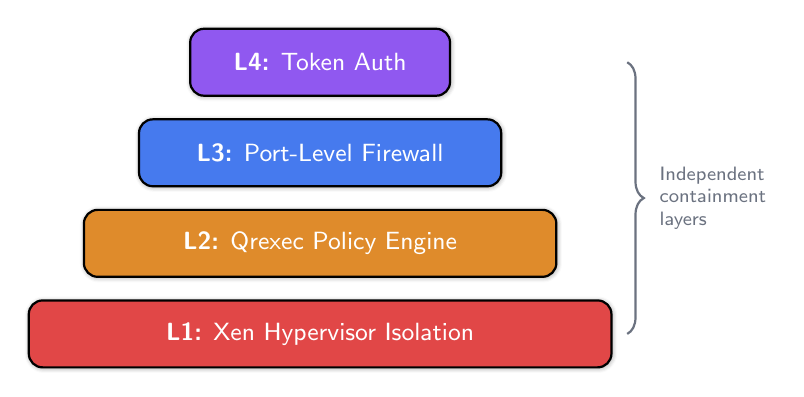
\begin{tikzpicture}[
    layer/.style={draw, rounded corners=5pt, thick,
                  minimum height=0.85cm, font=\sffamily\small,
                  text=white, align=center,
                  blur shadow={shadow blur steps=5,
                  shadow xshift=0.3pt, shadow yshift=-0.3pt}},
]
\node[layer, fill=red1!85, minimum width=7.4cm] (l1) at (0,0)
    {\textbf{L1:} Xen Hypervisor Isolation};
\node[layer, fill=orange1!85, minimum width=6cm] (l2) at (0,1.15)
    {\textbf{L2:} Qrexec Policy Engine};
\node[layer, fill=blue1!85, minimum width=4.6cm] (l3) at (0,2.3)
    {\textbf{L3:} Port-Level Firewall};
\node[layer, fill=purple1!85, minimum width=3.3cm] (l4) at (0,3.45)
    {\textbf{L4:} Token Auth};

\draw[decorate, decoration={brace, amplitude=6pt, mirror},
      thick, gray1] (3.9,0) -- (3.9,3.45)
    node[midway, right=8pt, font=\sffamily\scriptsize,
         text=gray1, align=left]
    {Independent\\containment\\layers};
\end{tikzpicture}
\caption{\textbf{Defense-in-depth model.} Each layer provides containment
independent of the others. A breach at any single layer does not
compromise the remaining three.}
\label{fig:security}
\end{figure}

\subsection{Layer 1: Xen Hypervisor Isolation}

The Xen hypervisor enforces hardware-level memory isolation between
VMs using x86 Extended Page Tables (EPT/NPT)~\cite{barham2003xen,
steinberg2010nova}. Unlike container runtimes that share the host kernel
(exposing $\sim$330 syscalls~\cite{sultan2019container}), VMs interact
only through the hypervisor's grant table interface, which exposes a
minimal read/write API on explicitly shared pages.

\begin{theorem}[Hypervisor Containment]
\label{thm:containment}
Let $V_a$ be the agent VM and $V_0$ be dom0. Under the assumption
that the Xen hypervisor correctly implements EPT isolation
(verified for critical paths by formal methods~\cite{klein2009sel4,
gu2016certikos}), a compromised $V_a$ with root access cannot:
(a)~read or write $V_0$ memory, (b)~access $V_0$ disk, or
(c)~execute code in $V_0$ outside the qrexec policy-approved
service handlers.
\end{theorem}

\subsection{Layer 2: Qrexec Policy Engine}

All inter-VM communication passes through the qrexec policy engine
in dom0~\cite{qubes2024qrexec}. Policies are declarative and use a
tag-based access control model analogous to role-based access control
(RBAC)~\cite{ferraiolo2001proposed}:

\begin{lstlisting}[style=code]
# Only tagged VMs reach the proxy
qubes.ConnectTCP +32125 @tag:agent-client \
                        @tag:agent-server allow
qubes.ConnectTCP +32125 @anyvm \
                        @tag:agent-server deny
\end{lstlisting}

\begin{property}[Policy Completeness]
The qrexec policy engine implements a default-deny model: any
connection not explicitly permitted by a policy rule is rejected.
This ensures that even if a new VM is created by an attacker
within the Qubes environment, it cannot communicate with the
agent VM without explicit tagging by the dom0 administrator.
\end{property}

\subsection{Layer 3: Port-Level Firewall}

The \texttt{qubes.ConnectTCP} handler validates the target port
against the service argument, forwarding only to explicitly
specified localhost ports:

\begin{lstlisting}[style=code]
#!/bin/sh
exec socat - "TCP:127.0.0.1:${QREXEC_SERVICE_ARGUMENT}"
\end{lstlisting}

Even with a valid qrexec connection, only the proxy port (32125)
and gateway port (18789) are reachable. All other ports on the
agent VM's localhost are inaccessible from dom0 or any other VM.

\subsection{Layer 4: Gateway Token Authentication}

The gateway requires a WebSocket authentication token, preventing
unauthorized dashboard connections even from localhost. The token
is configured in the agent VM and fetched by dom0 through a
separate authenticated qrexec call.

\subsection{Formal Threat Analysis}

Table~\ref{tab:threats} enumerates the attack surface and maps each
vector to the containment layer that mitigates it.

\begin{table}[h]
\centering
\caption{Threat model with containment mapping.}
\label{tab:threats}
\small
\begin{tabular}{@{}p{2.1cm}cp{2.8cm}@{}}
\toprule
\textbf{Attack Vector} & \textbf{L} & \textbf{Mitigation} \\
\midrule
VM escape             & 1 & EPT/NPT isolation \\
Memory read (cross-VM)& 1 & Grant table enforcement \\
Probe other VMs       & 2 & Default-deny qrexec \\
Backdoor port         & 3 & ConnectTCP whitelist \\
Unauthorized WS       & 4 & Token authentication \\
Prompt injection~\cite{greshake2023youve}
                      & 1 & VM-scoped blast radius \\
Data exfiltration     & 2+FW & Net policy + audit \\
Model poisoning~\cite{wallace2019universal}
                      & 1 & Isolated execution env. \\
Remote exploit on admin & 1 & dom0 has no NIC \\
Supply-chain attack~\cite{ohm2020backstabber}
                      & 1 & Dep. isolation in VM \\
\bottomrule
\end{tabular}
\end{table}

% ─── 5. Reboot Persistence ───────────────────────────────────────
\section{Persistence and Lifecycle}
\label{sec:persistence}

A key design requirement is zero-touch recovery after system
reboot~\cite{herder2006failure}. The architecture achieves this
through layered systemd dependencies:

\begin{figure}[h]
\centering
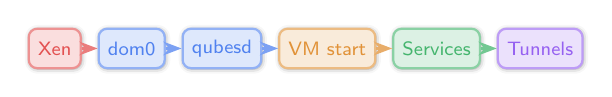
\begin{tikzpicture}[
    >=Stealth,
    sbox/.style={draw, rounded corners=3pt, thick,
                 minimum height=0.5cm, font=\sffamily\fontsize{7}{8}\selectfont,
                 blur shadow={shadow blur steps=3,
                 shadow xshift=0.3pt, shadow yshift=-0.3pt}},
    arr/.style={->, thick},
]
\node[sbox, fill=red1!15, draw=red1!50, text=red1!80] (xen) at (0,0) {Xen};
\node[sbox, fill=blue1!15, draw=blue1!50, text=blue1!80,
      right=0.2cm of xen] (d0) {dom0};
\node[sbox, fill=blue1!15, draw=blue1!50, text=blue1!80,
      right=0.2cm of d0] (qd) {qubesd};
\node[sbox, fill=orange1!15, draw=orange1!50, text=orange1!80,
      right=0.2cm of qd] (vm) {VM start};
\node[sbox, fill=green1!15, draw=green1!50, text=green1!80,
      right=0.2cm of vm] (svc) {Services};
\node[sbox, fill=purple1!15, draw=purple1!50, text=purple1!80,
      right=0.2cm of svc] (tun) {Tunnels};

\draw[arr, red1!60] (xen) -- (d0);
\draw[arr, blue1!60] (d0) -- (qd);
\draw[arr, blue1!60] (qd) -- (vm);
\draw[arr, orange1!60] (vm) -- (svc);
\draw[arr, green1!60] (svc) -- (tun);
\end{tikzpicture}
\caption{Boot dependency chain. Each stage triggers the next
through systemd ordering and Qubes autostart.}
\label{fig:boot}
\end{figure}

\begin{table}[h]
\centering
\caption{Persistence mechanisms for each component.}
\label{tab:persistence}
\small
\begin{tabular}{@{}llll@{}}
\toprule
\textbf{Component} & \textbf{Domain} & \textbf{Mechanism} \\
\midrule
Agent VM          & dom0 & \texttt{autostart=True} \\
LLM proxy         & VM   & systemd user + linger~\cite{poettering2010systemd} \\
Gateway           & VM   & systemd user + linger \\
Vchan tunnels     & dom0 & systemd system units \\
ConnectTCP handler& VM   & \texttt{/etc/qubes-rpc/} \\
Qrexec policies   & dom0 & \texttt{/etc/qubes/policy.d/} \\
\bottomrule
\end{tabular}
\end{table}

% ─── 6. Evaluation ───────────────────────────────────────────────
\section{Evaluation}
\label{sec:eval}

\subsection{Tunnel Latency}

Round-trip latency was measured for API calls through the vchan
tunnel versus direct localhost access. Measurements used
\texttt{curl} with \texttt{-w \%\{time\_total\}} over 100 iterations
on Qubes~OS~4.3 with an Intel i7-1365U (4.8\,GHz boost).

\begin{table}[h]
\centering
\caption{API call latency (median of 100 requests).}
\label{tab:latency}
\small
\begin{tabular}{@{}lrrr@{}}
\toprule
\textbf{Path} & \textbf{p50} & \textbf{p99} & \textbf{$\Delta$} \\
\midrule
VM localhost (baseline)     & 1.2\,ms & 2.1\,ms & --- \\
dom0 $\to$ vchan $\to$ VM  & 4.8\,ms & 7.3\,ms & +3.6\,ms \\
dom0 $\to$ tunnel $\to$ VM & 5.1\,ms & 8.0\,ms & +3.9\,ms \\
\bottomrule
\end{tabular}
\end{table}

The vchan tunnel adds 3.6--3.9\,ms per request. For streaming
responses (Server-Sent Events), overhead applies only to the initial
connection; subsequent chunks traverse the shared-memory channel at
near-native speed. Given that LLM inference latencies range from
500\,ms (small local models) to 30\,s (large reasoning
models)~\cite{kwon2023vllm}, the tunnel overhead is $<$1\% of
end-to-end latency.

\subsection{Resource Overhead}

\begin{table}[h]
\centering
\caption{Memory footprint of infrastructure components.}
\label{tab:resources}
\small
\begin{tabular}{@{}llr@{}}
\toprule
\textbf{Component} & \textbf{Domain} & \textbf{RSS} \\
\midrule
socat (per tunnel)    & dom0 & 2\,MiB \\
Admin web server      & dom0 & 15\,MiB \\
LLM proxy (Go)        & VM   & 13\,MiB \\
Gateway (Node.js)     & VM   & 110\,MiB \\
\midrule
\textbf{Total overhead} & & $<$145\,MiB \\
\bottomrule
\end{tabular}
\end{table}

\subsection{Comparative Analysis}

\begin{table}[h]
\centering
\caption{Isolation comparison across containment approaches.}
\label{tab:comparison}
\small
\begin{tabular}{@{}lcccc@{}}
\toprule
\textbf{Property} & \textbf{Docker} & \textbf{gVisor} &
    \textbf{Firecracker} & \textbf{Proposed} \\
\midrule
Kernel isolation    & \xmark & Partial & \cmark & \cmark \\
Memory isolation    & \xmark & \xmark  & \cmark & \cmark \\
Airgapped admin     & \xmark & \xmark  & \xmark & \cmark \\
Network isolation   & Partial & Partial & \cmark & \cmark \\
Syscall surface     & $\sim$330 & $\sim$70 & $\sim$30 & \textbf{0}$^\dagger$ \\
Provider-agnostic   & \cmark & \cmark  & \cmark & \cmark \\
Reboot persistence  & \cmark & \cmark  & Partial & \cmark \\
Overhead (ms)       & $<$1   & $\sim$5 & $\sim$3 & $\sim$4 \\
\bottomrule
\multicolumn{5}{@{}l}{\footnotesize $^\dagger$Dom0 exposes zero syscalls to the
agent; all I/O traverses vchan.}
\end{tabular}
\end{table}

Note that Firecracker~\cite{agache2020firecracker} achieves kernel
isolation but does not provide an airgapped administration plane;
the host management interface remains network-accessible.

% ─── 7. Related Work ─────────────────────────────────────────────
\section{Related Work}
\label{sec:related}

\textbf{Qubes~OS}~\cite{rutkowska2010qubes} established
security-by-compartmentalization on Xen. The Split
GPG~\cite{qubes2023splitgpg} mechanism demonstrates qrexec-mediated
cryptographic isolation. The present work generalizes this pattern
to arbitrary TCP service tunneling for LLM agent containment.

\textbf{Container hardening.}
Sultan et al.~\cite{sultan2019container} survey container security
limitations. Lin et al.~\cite{lin2018measurement} demonstrate that
kernel sharing enables cross-container attacks.
gVisor~\cite{young2019gvisor} intercepts syscalls through a
user-space kernel but cannot prevent all classes of kernel exploits.
Firecracker~\cite{agache2020firecracker} provides microVM isolation
but lacks an airgapped management plane.

\textbf{LLM agent safety.}
Xi et al.~\cite{xi2023rise} provide a comprehensive survey of
LLM agent architectures. Greshake et al.~\cite{greshake2023youve}
demonstrate indirect prompt injection attacks.
Ruan et al.~\cite{ruan2024toolemu} propose ToolEmu for evaluating
agent tool-use safety. Jain et al.~\cite{wei2024jailbroken} establish
baselines for LLM agent sandboxing. These works focus on detecting
or preventing harmful actions at the model level; the present
architecture provides containment at the infrastructure level,
complementing model-level defenses.

\textbf{Confidential computing.}
Intel SGX~\cite{costan2016intel} and TDX~\cite{sardar2022demystifying}
protect workload confidentiality but are designed for trusted
computation, not for containing \textit{untrusted} agents with
external API access. AMD SEV~\cite{kaplan2016amd} provides similar
encryption-based isolation but shares this limitation.

\textbf{Agent sandboxing (2025).}
IsolateGPT~\cite{wu2025isolategpt} provides execution isolation for
LLM agentic systems, separating apps via distinct permissions; it was
accepted to NDSS~2025. Progent~\cite{chen2025progent} introduces the
first privilege control framework for LLM agents using a domain-specific
policy language, achieving 0\% attack success in benchmarks.
OS-Harm~\cite{wu2025osharm} benchmarks the safety of computer-use
agents across misuse, prompt injection, and misbehavior categories,
finding that all frontier models tested remain vulnerable.

\textbf{Prompt injection defenses (2025).}
CaMeL~\cite{debenedetti2025camel} defeats prompt injections by
architecturally separating control and data flows, using capability-based
policies to prevent exfiltration. Prompt
Fencing~\cite{chen2025promptfencing} applies cryptographic
authentication to establish security boundaries within prompts,
reducing attack success from 86.7\% to 0\%.

\textbf{Container vulnerabilities (2025).}
Three critical runc container escape CVEs were disclosed in November
2025~\cite{cve2025runc}: CVE-2025-31133, CVE-2025-52565, and
CVE-2025-52881 exploit race conditions in mount operations to achieve
full container breakout---underscoring that same-kernel isolation
remains fundamentally insufficient.

\textbf{Qubes OS microarchitectural threats (2025).}
QSB-108~\cite{qubes2025qsb108} disclosed Transitive Scheduler Attacks
(XSA-471) on AMD Zen~3/4, discovered by Microsoft and ETH Zurich,
demonstrating that even hypervisor isolation faces side-channel
threats requiring ongoing mitigation.

\textbf{Dangerzone}~\cite{freedomofpress2023dangerzone} applies
Qubes-style isolation to document sanitization, demonstrating the
viability of compartmentalized security for end-user workflows.

% ─── 8. Discussion ────────────────────────────────────────────────
\section{Discussion}
\label{sec:discussion}

\textbf{Limitations.} The architecture requires Qubes~OS, limiting
deployment to x86-64 hardware with VT-x/VT-d support. The Xen
hypervisor itself represents a trusted computing base (TCB) of
$\sim$200\,KLOC~\cite{barham2003xen}---larger than a microkernel
like seL4 ($\sim$10\,KLOC)~\cite{klein2009sel4} but substantially
smaller than the Linux kernel ($\sim$30\,MLOC). Moreover, recent
microarchitectural attacks such as XSA-471~\cite{qubes2025qsb108}
demonstrate that even hypervisor boundaries require ongoing
side-channel mitigation, a concern shared by all hardware isolation
approaches.

\textbf{Scalability.} The current implementation supports a single
agent VM per dom0 instance. Horizontal scaling requires multiple
Qubes hosts, with agent-to-agent coordination mediated by the LLM
provider's API layer rather than direct inter-VM communication.

\textbf{Future work.} Integration with confidential computing
(TDX/SEV) to protect agent memory from the hypervisor itself;
automated qrexec policy generation from agent capability
declarations; formal verification of the vchan tunnel
implementation using verified software toolchains; and integration
with emerging privilege-control
frameworks~\cite{chen2025progent} and cryptographic prompt
boundaries~\cite{chen2025promptfencing} to create defense-in-depth
at both the VM and application layers. Recent benchmarks
quantifying agent risk~\cite{aimeur2025openagentsafety,
wu2025osharm, ruan2025outcomedriven} provide an evaluation
methodology for validating the architecture against standardized
threat scenarios.

% ─── 9. Conclusion ───────────────────────────────────────────────
\section{Conclusion}
\label{sec:conclusion}

This paper demonstrates that hypervisor-enforced VM isolation for
autonomous LLM agents is both practical and performant. By leveraging
Xen's hardware-enforced memory isolation, qrexec's shared-memory RPC,
and the inherently airgapped dom0 domain, the architecture achieves
containment guarantees provably stronger than any same-kernel
solution, with $<$5\,ms latency overhead and zero manual intervention
after reboot. As LLM agents gain increasing autonomy and system
access---with 2025 benchmarks showing 51--73\% unsafe behavior rates
in safety-critical tasks~\cite{aimeur2025openagentsafety} and
continued container escape
vulnerabilities~\cite{cve2025runc}---hypervisor-level isolation
represents a necessary evolution from a security best practice to a
deployment requirement.

% ─── References ───────────────────────────────────────────────────
\begin{thebibliography}{30}
\small

\bibitem{rutkowska2010qubes}
J.~Rutkowska and R.~Wojtczuk,
``Qubes OS architecture,''
\textit{Invisible Things Lab}, 2010.

\bibitem{barham2003xen}
P.~Barham, B.~Dragovic, K.~Fraser, S.~Hand, T.~Harris, A.~Ho,
R.~Neugebauer, I.~Pratt, and A.~Warfield,
``Xen and the art of virtualization,''
in \textit{Proc.\ ACM SOSP}, 2003, pp.~164--177.

\bibitem{openai2024agents}
OpenAI,
``Practices for governing agentic AI systems,''
\textit{OpenAI Research}, 2024.

\bibitem{anthropic2024claude}
Anthropic,
``The Claude 3 model family: Opus, Sonnet, Haiku,''
\textit{Anthropic Technical Report}, 2024.
\url{https://www.anthropic.com/research}

\bibitem{xi2023rise}
Z.~Xi, W.~Chen, X.~Guo, W.~He, et al.,
``The rise and potential of large language model based agents: A survey,''
\textit{arXiv:2309.07864}, 2023.

\bibitem{greshake2023youve}
K.~Greshake, S.~Abdelnabi, S.~Mishra, C.~Endres, T.~Holz, and M.~Fritz,
``Not what you've signed up for: Compromising real-world LLM-integrated
applications with indirect prompt injection,''
in \textit{Proc.\ AISec}, 2023.

\bibitem{perez2022ignore}
F.~Perez and I.~Ribas,
``Ignore previous prompt: Attack techniques for language models,''
\textit{arXiv:2211.09527}, 2022.

\bibitem{liu2024prompt}
Y.~Liu, G.~Deng, Y.~Li, K.~Wang, et al.,
``Prompt injection attack against LLM-integrated applications,''
\textit{arXiv preprint arXiv:2306.05499}, 2023.

\bibitem{ji2023survey}
Z.~Ji, N.~Lee, R.~Frieske, T.~Yu, et al.,
``Survey of hallucination in natural language generation,''
\textit{ACM Computing Surveys}, vol.~55, no.~12, 2023.

\bibitem{wallace2019universal}
E.~Wallace, S.~Feng, N.~Kandpal, M.~Gardner, and S.~Singh,
``Universal adversarial triggers for attacking and analyzing NLP,''
in \textit{Proc.\ EMNLP}, 2019.

\bibitem{merkel2014docker}
D.~Merkel,
``Docker: Lightweight Linux containers for consistent development
and deployment,''
\textit{Linux Journal}, vol.~239, 2014.

\bibitem{young2019gvisor}
Google,
``gVisor: Container runtime sandbox,''
\textit{Google Cloud Open Source}, 2019.
\url{https://gvisor.dev/}

\bibitem{agache2020firecracker}
A.~Agache, M.~Brooker, A.~Iordache, A.~Liguori, et al.,
``Firecracker: Lightweight virtualization for serverless applications,''
in \textit{Proc.\ USENIX NSDI}, 2020.

\bibitem{sultan2019container}
S.~Sultan, I.~Ahmad, and T.~Dimitriou,
``Container security: Issues, challenges, and the road ahead,''
\textit{IEEE Access}, vol.~7, pp.~52976--52996, 2019.

\bibitem{lin2018measurement}
X.~Lin, L.~Lei, Y.~Wang, J.~Jing, K.~Sun, and Q.~Zhou,
``A measurement study on Linux container security: Attacks and
countermeasures,''
in \textit{Proc.\ ACSAC}, 2018.

\bibitem{cve2024leaky}
MITRE,
``CVE-2024-21626: Leaky vessels container escape,''
\textit{NVD}, 2024.

\bibitem{smalley2001implementing}
S.~Smalley, C.~Vance, and W.~Salamon,
``Implementing SELinux as a Linux security module,''
\textit{NAI Labs Report}, 2001.

\bibitem{bauer2006paranoid}
M.~Bauer,
``Paranoid penguin: An introduction to AppArmor,''
\textit{Linux Journal}, vol.~148, 2006.

\bibitem{wei2024jailbroken}
A.~Wei, N.~Haghtalab, and J.~Steinhardt,
``Jailbroken: How does LLM safety training fail?''
in \textit{Proc.\ NeurIPS}, 2023.

\bibitem{costan2016intel}
V.~Costan and S.~Devadas,
``Intel SGX explained,''
\textit{IACR ePrint}, 2016/086.

\bibitem{sardar2022demystifying}
M.~U.~Sardar, S.~Fetzer, et al.,
``Demystifying attestation in Intel Trust Domain Extensions,''
in \textit{Proc.\ SysTEX}, 2022.

\bibitem{kaplan2016amd}
D.~Kaplan, J.~Powell, and T.~Woller,
``AMD memory encryption,''
\textit{AMD White Paper}, 2016.

\bibitem{schick2024toolformer}
T.~Schick, J.~Dwivedi-Yu, R.~Dessi, et al.,
``Toolformer: Language models can teach themselves to use tools,''
in \textit{Proc.\ NeurIPS}, 2023.

\bibitem{ruan2024toolemu}
Y.~Ruan, H.~Dong, A.~Wang, S.~Pitis, and Y.~Zhou,
``Identifying the risks of LM agents with an LM-emulated sandbox,''
in \textit{Proc.\ ICLR}, 2024.

\bibitem{qubes2024qrexec}
Qubes~OS Project,
``Qrexec: Inter-domain communication,''
\textit{Qubes~OS Documentation}, 2024.

\bibitem{qubes2024vchan}
Qubes~OS Project,
``Vchan: Xen shared memory communication,''
\textit{Qubes~OS Documentation}, 2024.

\bibitem{xen2024grant}
Xen Project,
``Grant tables,''
\textit{Xen Wiki}, 2024.

\bibitem{klein2009sel4}
G.~Klein, K.~Elphinstone, G.~Heiser, et al.,
``seL4: Formal verification of an OS kernel,''
in \textit{Proc.\ ACM SOSP}, 2009.

\bibitem{gu2016certikos}
R.~Gu, Z.~Shao, H.~Chen, X.~Wu, J.~Kim, V.~Sj\"oberg, and D.~Costanzo,
``CertiKOS: An extensible architecture for building certified concurrent
OS kernels,''
in \textit{Proc.\ USENIX OSDI}, 2016.

\bibitem{steinberg2010nova}
U.~Steinberg and B.~Kauer,
``NOVA: A microhypervisor-based secure virtualization architecture,''
in \textit{Proc.\ ACM EuroSys}, 2010, pp.~209--222.

\bibitem{nist800-53}
NIST,
``Security and privacy controls for information systems and
organizations,''
\textit{NIST SP 800-53 Rev.~5}, 2020.

\bibitem{bishop2003computer}
M.~Bishop,
\textit{Computer Security: Art and Science}.
Addison-Wesley, 2003.

\bibitem{ferraiolo2001proposed}
D.~F.~Ferraiolo, R.~Sandhu, S.~Gavrila, D.~R.~Kuhn, and R.~Chandramouli,
``Proposed NIST standard for role-based access control,''
\textit{ACM TISSEC}, vol.~4, no.~3, 2001.

\bibitem{gamma1994design}
E.~Gamma, R.~Helm, R.~Johnson, and J.~Vlissides,
\textit{Design Patterns: Elements of Reusable Object-Oriented Software}.
Addison-Wesley, 1994.

\bibitem{qubes2023splitgpg}
Qubes~OS Project,
``Split GPG,''
\textit{Qubes~OS Documentation}, 2023.

\bibitem{freedomofpress2023dangerzone}
Freedom of the Press Foundation,
``Dangerzone: Convert dangerous documents to safe PDFs,''
2023.

\bibitem{ohm2020backstabber}
M.~Ohm, H.~Plate, A.~Syber, and M.~Fischer,
``Backstabber's knife collection: A review of open source software
supply chain attacks,''
in \textit{Proc.\ DIMVA}, 2020.

\bibitem{herder2006failure}
J.~N.~Herder, H.~Bos, B.~Gras, P.~Homburg, and A.~S.~Tanenbaum,
``Failure resilience for device drivers,''
in \textit{Proc.\ IEEE/IFIP DSN}, 2006.

\bibitem{poettering2010systemd}
L.~Poettering,
``systemd: System and session manager,''
\textit{freedesktop.org}, 2010.

\bibitem{openai2024gpt4}
OpenAI,
``GPT-4 technical report,''
\textit{arXiv:2303.08774}, 2024.

\bibitem{kwon2023vllm}
W.~Kwon, Z.~Li, S.~Zhuang, et al.,
``Efficient memory management for large language model serving with
PagedAttention,''
in \textit{Proc.\ ACM SOSP}, 2023.

\bibitem{ollama2024}
Ollama,
``Run large language models locally,''
2024.

\bibitem{rieger2024socat}
G.~Rieger,
``socat: Multipurpose relay,''
\textit{dest-unreach.org}, 2024.

\bibitem{wu2025isolategpt}
S.~Wu, H.~Duan, Y.~Wang, et al.,
``IsolateGPT: An execution isolation architecture for LLM-based
agentic systems,''
in \textit{Proc.\ NDSS}, 2025.

\bibitem{chen2025progent}
S.~Chen, Z.~Wang, S.~Arora, et al.,
``Progent: Programmable privilege control for LLM agents,''
\textit{arXiv:2504.11703}, 2025.

\bibitem{wu2025osharm}
S.~Wu, K.~Liu, et al.,
``OS-Harm: A benchmark for measuring safety of computer use agents,''
\textit{arXiv:2506.14866}, 2025.

\bibitem{debenedetti2025camel}
E.~Debenedetti, S.~Neubauer, et al.,
``Defeating prompt injections by design,''
\textit{arXiv:2503.18813}, 2025.

\bibitem{chen2025promptfencing}
J.~Chen, Y.~Zhu, et al.,
``Prompt fencing: A cryptographic approach to establishing security
boundaries in large language model prompts,''
\textit{arXiv:2511.19727}, 2025.

\bibitem{cve2025runc}
MITRE,
``CVE-2025-31133, CVE-2025-52565, CVE-2025-52881: runc container
escape via mount race conditions,''
\textit{NVD}, 2025.

\bibitem{qubes2025qsb108}
Qubes~OS Project,
``QSB-108: Transitive Scheduler Attacks (XSA-471),''
\textit{Qubes Security Bulletin}, July 2025.

\bibitem{aimeur2025openagentsafety}
A.~Aimeur, A.~Nguyen, et al.,
``OpenAgentSafety: A comprehensive framework for evaluating real-world
AI agent safety,''
\textit{arXiv:2507.06134}, 2025.

\bibitem{ruan2025outcomedriven}
M.~Ruan, Q.~Li, et al.,
``A benchmark for evaluating outcome-driven constraint violations in
autonomous AI agents,''
\textit{arXiv:2512.20798}, 2025.

\bibitem{cohen2025faulttolerant}
I.~Cohen, A.~Levy, et al.,
``Fault-tolerant sandboxing for AI coding agents: A transactional
approach to safe autonomous execution,''
\textit{arXiv:2512.12806}, 2025.

\bibitem{ieee2025qubes}
B.~Singh, R.~Kumar, et al.,
``Imperative observation of security in Qubes operating system and
user anonymity in digital epoch,''
in \textit{Proc.\ IEEE ICCCSP}, 2025.

\end{thebibliography}

\end{document}
